\newthought{Lorum ipsum} sit dolor amet.\citefix{church1932}
\lipsum[2-3]

\begin{marginfigure}
	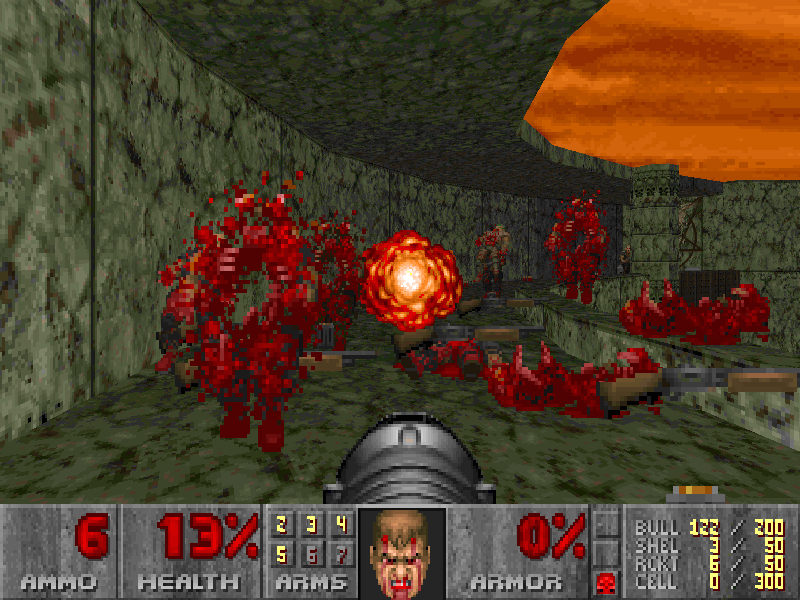
\includegraphics[width=6cm]{res/game_screens/doom/doom.png}
	\caption[A screen from \emph{Ultimate Doom}.]{A screen from \emph{Ultimate Doom} (1995). Extended caption etc.}
	\label{fig:doom}
\end{marginfigure}

\lipsum[4]

\section{Typesetting Haskell}

Lambda\TeX\ is written for \TeX\ rather than \LaTeX, and so works a little differently from how you might expect. It is designed to typeset Literate Haskell documents and so uses an angle brace to denote a haskell line:

>this is a Haskell line
>data List a = Cons a |Empty

To control the spacing and other parameters around these lines I have made a \emph{haskell} environment to be used like this.

\vspace{-0.5em}
\begin{listing}{list:reduce}{The \emph{reduce} function}{The \scalenote{"reduce"} function. Extended caption.}{}
\end{listing}\vspace{-1.5em}

\functions(reduce)
\begin{haskell}
>reduce :: (state -> alphabet -> state) -> state -> [alphabet] -> state
>reduce delta q0 []     = q0

\marginnote{\anote This definition uses pattern matching on the string being passed to split it into head and tail parts; ie the pattern \scalenote{"(x:xs)"} results in \scalenote{"x"} being the character at the head of the list and \scalenote{"xs"} the remaining list. }\vspace{-1.7em}
>reduce delta q0 (x:xs) = reduce delta (delta q0 x) xs

\end{haskell}
\noindent
The function command is to tell Lambda\TeX\ the names of functions as it couldn't otherwise work them out without a full Haskell parser. The lack of extra newlines around the end of the haskell environment and the \textbackslash noindent is required. The example above also shows how to embed a code annotation as a margin note. 

Inline haskell code is put between double tick marks ie "reduce delta q0". (Use a single tick twice for a normal closing quotation mark.) 

Lastly, Lambda\TeX\ will not react to normal text scaling commands as these are part of \LaTeX, so a scaling command must be added when setting Haskell within sidenotes or anywhere with a different text size.

Lastly, please get into the habit of indexing.\index{indexing}
